% Plantilla para un Trabajo Fin de Grado de la Universidad de Granada,
% adaptada para el Doble Grado en Ingeniería Informática y Matemáticas.
%
%  Autor: Mario Román.
%  Licencia: GNU GPLv2.
%
% Esta plantilla es una adaptación al castellano de la plantilla
% classicthesis de André Miede, que puede obtenerse en:
%  https://ctan.org/tex-archive/macros/latex/contrib/classicthesis?lang=en
% La plantilla original se licencia en GNU GPLv2.
%
% Esta plantilla usa símbolos de la Universidad de Granada sujetos a la normativa
% de identidad visual corporativa, que puede encontrarse en:
% http://secretariageneral.ugr.es/pages/ivc/normativa
%
% La compilación se realiza con las siguientes instrucciones:
%   pdflatex --shell-escape main.tex
%   bibtex main
%   pdflatex --shell-escape main.tex
%   pdflatex --shell-escape main.tex

% Opciones del tipo de documento
\documentclass[twoside,openright,titlepage,numbers=noenddot,openany,headinclude,footinclude=true,
cleardoublepage=empty,abstractoff,BCOR=5mm,paper=a4,fontsize=12pt,main=spanish]{scrreprt}

% Paquetes de latex que se cargan al inicio. Cubren la entrada de
% texto, gráficos, código fuente y símbolofs.
\usepackage[utf8]{inputenc}
\usepackage[T1]{fontenc}
\usepackage{fixltx2e}
\usepackage{graphicx} % Inclusión de imágenes.
\usepackage{grffile}  % Distintos formatos para imágenes.
\usepackage{longtable} % Tablas multipágina.
\usepackage{wrapfig} % Coloca texto alrededor de una figura.
\usepackage{rotating}
\usepackage[normalem]{ulem}
\usepackage{amsmath}
\usepackage{dsfont}
\usepackage{textcomp}
\usepackage{amssymb}
\usepackage{capt-of}
\usepackage[colorlinks=true]{hyperref}
\usepackage{tikz} % Diagramas conmutativos.
\usepackage{minted} % Código fuente.
\usepackage[T1]{fontenc}
\usepackage[numbers]{natbib}

% PAQUETE MIO

\usepackage{float}

% Plantilla classicthesis
\usepackage[beramono,eulerchapternumbers,linedheaders,parts,a5paper,dottedtoc,
manychapters,pdfspacing]{classicthesis}

% Geometría y espaciado de párrafos.
\setcounter{secnumdepth}{0}
\usepackage{enumitem}
\setitemize{noitemsep,topsep=0pt,parsep=0pt,partopsep=0pt}
\setlist[enumerate]{topsep=0pt,itemsep=-1ex,partopsep=1ex,parsep=1ex}
\usepackage[top=1in, bottom=1.5in, left=1in, right=1in]{geometry}
\setlength\itemsep{0em}
\setlength{\parindent}{0pt}
\usepackage{parskip}

% Profundidad de la tabla de contenidos.
\setcounter{secnumdepth}{3}

% Usa el paquete minted para mostrar trozos de código.
% Pueden seleccionarse el lenguaje apropiado y el estilo del código.
\usepackage{minted}
\usemintedstyle{colorful}
\setminted{fontsize=\small}
\setminted[haskell]{linenos=false,fontsize=\small}
\renewcommand{\theFancyVerbLine}{\sffamily\textcolor[rgb]{0.5,0.5,1.0}{\oldstylenums{\arabic{FancyVerbLine}}}}

% Path para las imágenes
\graphicspath{{figures/}}

% Archivos de configuración.
%------------------------
% Bibliotecas para matemáticas de latex
%------------------------
\usepackage{amsthm}
\usepackage{amsmath}
\usepackage{tikz}
\usepackage{tikz-cd}
\usetikzlibrary{shapes,fit}
\usepackage{bussproofs}
\EnableBpAbbreviations{}
\usepackage{mathtools}
\usepackage{scalerel}
\usepackage{stmaryrd}

%------------------------
% Estilos para los teoremas
%------------------------
\theoremstyle{plain}
\newtheorem{theorem}{Teorema}
\newtheorem{proposition}{Proposición}
\newtheorem{lemma}{Lema}
\newtheorem{corollary}{Corolario}

\theoremstyle{definition}
\newtheorem{definition}{Definición}
\newtheorem{postulate}{Postulado}
\newtheorem*{postulate 3'}{Postulate 3'}
\newtheorem*{postulate 2'}{Projective Measurement}


% Comento estas lineas originales intentando que diga dem
%\renewenvironment{proof}{{\bfseries Proof.}}{\qed}

% Change the proof style so it's in English and add \qed at the end.
%\renewenvironment{proof}{{\bfseries Proof.}}{\qed}

% Añadido por mi intentando que pone "Demostración" y no "Proof"
\renewenvironment{proof}{{\bfseries Demostración.}}{\qed}
\renewenvironment{proof}{{\bfseries Demostración.}}{\qed}
% hasta aqui

\theoremstyle{remark}
\newtheorem{remark}{Remark}
\newtheorem{exampleth}{Ejemplo}

\begingroup\makeatletter\@for\theoremstyle:=definition,remark,plain\do{\expandafter\g@addto@macro\csname th@\theoremstyle\endcsname{\addtolength\thm@preskip\parskip}}\endgroup

%------------------------
% Macros
% ------------------------

\newcommand*{\C}{\mathds{C}}
\newcommand*{\ra}{\rangle}
\newcommand*{\la}{\langle}

% Para poner sonrisa sobre puntos suspensivos. Uso: \overplace{n}{\dotsc}
\newcommand{\overplace}[2]{%
	\overset{\substack{#1\\\smile}}{#2}%
}  % En macros.tex se almacenan las opciones y comandos para escribir matemáticas.
% ****************************************************************************************************
% classicthesis-config.tex 
% formerly known as loadpackages.sty, classicthesis-ldpkg.sty, and classicthesis-preamble.sty 
% Use it at the beginning of your ClassicThesis.tex, or as a LaTeX Preamble 
% in your ClassicThesis.{tex,lyx} with % ****************************************************************************************************
% classicthesis-config.tex 
% formerly known as loadpackages.sty, classicthesis-ldpkg.sty, and classicthesis-preamble.sty 
% Use it at the beginning of your ClassicThesis.tex, or as a LaTeX Preamble 
% in your ClassicThesis.{tex,lyx} with % ****************************************************************************************************
% classicthesis-config.tex 
% formerly known as loadpackages.sty, classicthesis-ldpkg.sty, and classicthesis-preamble.sty 
% Use it at the beginning of your ClassicThesis.tex, or as a LaTeX Preamble 
% in your ClassicThesis.{tex,lyx} with \input{classicthesis-config}
% ****************************************************************************************************  
% If you like the classicthesis, then I would appreciate a postcard. 
% My address can be found in the file ClassicThesis.pdf. A collection 
% of the postcards I received so far is available online at 
% http://postcards.miede.de
% ****************************************************************************************************


% ****************************************************************************************************
% 0. Set the encoding of your files. UTF-8 is the only sensible encoding nowadays. If you can't read
% äöüßáéçèê∂åëæƒÏ€ then change the encoding setting in your editor, not the line below. If your editor
% does not support utf8 use another editor!
% ****************************************************************************************************
\PassOptionsToPackage{utf8x}{inputenc}
	\usepackage{inputenc}

% ****************************************************************************************************
% 1. Configure classicthesis for your needs here, e.g., remove "drafting" below 
% in order to deactivate the time-stamp on the pages
% ****************************************************************************************************
\PassOptionsToPackage{eulerchapternumbers,listings,drafting,%
		pdfspacing,%floatperchapter,%linedheaders,%
                subfig,beramono,eulermath,parts,dottedtoc}{classicthesis}                                        
% ********************************************************************
% Available options for classicthesis.sty 
% (see ClassicThesis.pdf for more information):
% drafting
% parts nochapters linedheaders
% eulerchapternumbers beramono eulermath pdfspacing minionprospacing
% tocaligned dottedtoc manychapters
% listings floatperchapter subfig
% ********************************************************************

% ****************************************************************************************************
% 2. Personal data and user ad-hoc commands
% ****************************************************************************************************
\newcommand{\myTitle}{Practica 2\xspace}
\newcommand{\mySubtitle}{An Homage to The Elements of Typographic Style\xspace}
\newcommand{\myDegree}{Doktor-Ingenieur (Dr.-Ing.)\xspace}
\newcommand{\myName}{André Miede\xspace}
\newcommand{\myProf}{Put name here\xspace}
\newcommand{\myOtherProf}{Put name here\xspace}
\newcommand{\mySupervisor}{Put name here\xspace}
\newcommand{\myFaculty}{Put data here\xspace}
\newcommand{\myDepartment}{Put data here\xspace}
\newcommand{\myUni}{Put data here\xspace}
\newcommand{\myLocation}{Saarbrücken\xspace}
\newcommand{\myTime}{September 2015\xspace}
%\newcommand{\myVersion}{version 4.2\xspace}

% ********************************************************************
% Setup, finetuning, and useful commands
% ********************************************************************
\newcounter{dummy} % necessary for correct hyperlinks (to index, bib, etc.)
\newlength{\abcd} % for ab..z string length calculation
\providecommand{\mLyX}{L\kern-.1667em\lower.25em\hbox{Y}\kern-.125emX\@}
\newcommand{\ie}{i.\,e.}
\newcommand{\Ie}{I.\,e.}
\newcommand{\eg}{e.\,g.}
\newcommand{\Eg}{E.\,g.} 
% ****************************************************************************************************


% ****************************************************************************************************
% 3. Loading some handy packages
% ****************************************************************************************************
% ******************************************************************** 
% Packages with options that might require adjustments
% ******************************************************************** 
%\PassOptionsToPackage{ngerman,american}{babel}   % change this to your language(s)
% Spanish languages need extra options in order to work with this template
% \PassOptionsToPackage{es-lcroman,spanish}{babel}
\usepackage[main=spanish]{babel}

%\usepackage{csquotes}
% \PassOptionsToPackage{%
%     %backend=biber, %instead of bibtex
% 	backend=bibtex8,bibencoding=ascii,%
% 	language=auto,%
% 	style=alpha,%
%     %style=authoryear-comp, % Author 1999, 2010
%     %bibstyle=authoryear,dashed=false, % dashed: substitute rep. author with ---
%     sorting=nyt, % name, year, title
%     maxbibnames=10, % default: 3, et al.
%     %backref=true,%
%     natbib=true % natbib compatibility mode (\citep and \citet still work)
% }{biblatex}
%     \usepackage{biblatex}

% \PassOptionsToPackage{fleqn}{amsmath}       % math environments and more by the AMS 
%     \usepackage{amsmath}

% ******************************************************************** 
% General useful packages
% ******************************************************************** 
\PassOptionsToPackage{T1}{fontenc} % T2A for cyrillics
    \usepackage{fontenc}     
\usepackage{textcomp} % fix warning with missing font shapes
\usepackage{scrhack} % fix warnings when using KOMA with listings package          
\usepackage{xspace} % to get the spacing after macros right  
\usepackage{mparhack} % get marginpar right
\usepackage{fixltx2e} % fixes some LaTeX stuff --> since 2015 in the LaTeX kernel (see below)
%\usepackage[latest]{latexrelease} % will be used once available in more distributions (ISSUE #107)
\PassOptionsToPackage{printonlyused,smaller}{acronym} 
    \usepackage{acronym} % nice macros for handling all acronyms in the thesis
    %\renewcommand{\bflabel}[1]{{#1}\hfill} % fix the list of acronyms --> no longer working
    %\renewcommand*{\acsfont}[1]{\textsc{#1}} 
    \renewcommand*{\aclabelfont}[1]{\acsfont{#1}}
% ****************************************************************************************************


% ****************************************************************************************************
% 4. Setup floats: tables, (sub)figures, and captions
% ****************************************************************************************************
\usepackage{tabularx} % better tables
    \setlength{\extrarowheight}{3pt} % increase table row height
\newcommand{\tableheadline}[1]{\multicolumn{1}{c}{\spacedlowsmallcaps{#1}}}
\newcommand{\myfloatalign}{\centering} % to be used with each float for alignment
\usepackage{caption}
% Thanks to cgnieder and Claus Lahiri
% http://tex.stackexchange.com/questions/69349/spacedlowsmallcaps-in-caption-label
% [REMOVED DUE TO OTHER PROBLEMS, SEE ISSUE #82]    
%\DeclareCaptionLabelFormat{smallcaps}{\bothIfFirst{#1}{~}\MakeTextLowercase{\textsc{#2}}}
%\captionsetup{font=small,labelformat=smallcaps} % format=hang,
\captionsetup{font=small} % format=hang,
\usepackage{subfig}  
% ****************************************************************************************************


% ****************************************************************************************************
% 5. Setup code listings
% ****************************************************************************************************
% \usepackage{listings} 
% %\lstset{emph={trueIndex,root},emphstyle=\color{BlueViolet}}%\underbar} % for special keywords
% \lstset{language={Haskell},morekeywords={PassOptionsToPackage,selectlanguage},keywordstyle=\color{RoyalBlue},basicstyle=\small\ttfamily,commentstyle=\color{Green}\ttfamily,stringstyle=\rmfamily,numbers=none,numberstyle=\scriptsize,stepnumber=5,numbersep=8pt,showstringspaces=false,breaklines=true,belowcaptionskip=.75\baselineskip} 
% ****************************************************************************************************             


% ****************************************************************************************************
% 6. PDFLaTeX, hyperreferences and citation backreferences
% ****************************************************************************************************
% ********************************************************************
% Using PDFLaTeX
% ********************************************************************
\PassOptionsToPackage{pdftex,hyperfootnotes=false,pdfpagelabels}{hyperref}
    \usepackage{hyperref}  % backref linktocpage pagebackref
\pdfcompresslevel=9
\pdfadjustspacing=1 
\PassOptionsToPackage{pdftex}{graphicx}
    \usepackage{graphicx} 
 

% ********************************************************************
% Hyperreferences
% ********************************************************************
\hypersetup{%
    %draft, % = no hyperlinking at all (useful in b/w printouts)
    colorlinks=true, linktocpage=true, pdfstartpage=3, pdfstartview=FitV,%
    % uncomment the following line if you want to have black links (e.g., for printing)
    %colorlinks=false, linktocpage=false, pdfstartpage=3, pdfstartview=FitV, pdfborder={0 0 0},%
    breaklinks=true, pdfpagemode=UseNone, pageanchor=true, pdfpagemode=UseOutlines,%
    plainpages=false, bookmarksnumbered, bookmarksopen=true, bookmarksopenlevel=1,%
    hypertexnames=true, pdfhighlight=/O,%nesting=true,%frenchlinks,%
    urlcolor=webbrown, linkcolor=RoyalBlue, citecolor=webgreen, %pagecolor=RoyalBlue,%
    %urlcolor=Black, linkcolor=Black, citecolor=Black, %pagecolor=Black,%
    pdftitle={\myTitle},%
    pdfauthor={\textcopyright\ \myName, \myUni, \myFaculty},%
    pdfsubject={},%
    pdfkeywords={},%
    pdfcreator={pdfLaTeX},%
    pdfproducer={LaTeX with hyperref and classicthesis}%
}   

% ********************************************************************
% Setup autoreferences
% ********************************************************************
% There are some issues regarding autorefnames
% http://www.ureader.de/msg/136221647.aspx
% http://www.tex.ac.uk/cgi-bin/texfaq2html?label=latexwords
% you have to redefine the makros for the 
% language you use, e.g., american, ngerman
% (as chosen when loading babel/AtBeginDocument)
% ********************************************************************
\makeatletter
\@ifpackageloaded{babel}%
    {%
       \addto\extrasamerican{%
			\renewcommand*{\figureautorefname}{Figure}%
			\renewcommand*{\tableautorefname}{Table}%
			\renewcommand*{\partautorefname}{Part}%
			\renewcommand*{\chapterautorefname}{Chapter}%
			\renewcommand*{\sectionautorefname}{Section}%
			\renewcommand*{\subsectionautorefname}{Section}%
			\renewcommand*{\subsubsectionautorefname}{Section}%     
                }%
       \addto\extrasngerman{% 
			\renewcommand*{\paragraphautorefname}{Absatz}%
			\renewcommand*{\subparagraphautorefname}{Unterabsatz}%
			\renewcommand*{\footnoteautorefname}{Fu\"snote}%
			\renewcommand*{\FancyVerbLineautorefname}{Zeile}%
			\renewcommand*{\theoremautorefname}{Theorem}%
			\renewcommand*{\appendixautorefname}{Anhang}%
			\renewcommand*{\equationautorefname}{Gleichung}%        
			\renewcommand*{\itemautorefname}{Punkt}%
                }%  
            % Fix to getting autorefs for subfigures right (thanks to Belinda Vogt for changing the definition)
            \providecommand{\subfigureautorefname}{\figureautorefname}%             
    }{\relax}
\makeatother


% ****************************************************************************************************
% 7. Last calls before the bar closes
% ****************************************************************************************************
% ********************************************************************
% Development Stuff
% ********************************************************************
\listfiles
%\PassOptionsToPackage{l2tabu,orthodox,abort}{nag}
%   \usepackage{nag}
%\PassOptionsToPackage{warning, all}{onlyamsmath}
%   \usepackage{onlyamsmath}

% ********************************************************************
% Last, but not least...
% ********************************************************************
\usepackage{classicthesis} 
% ****************************************************************************************************


% ****************************************************************************************************
% 8. Further adjustments (experimental)
% ****************************************************************************************************
% ********************************************************************
% Changing the text area
% ********************************************************************
%\linespread{1.05} % a bit more for Palatino
%\areaset[current]{312pt}{761pt} % 686 (factor 2.2) + 33 head + 42 head \the\footskip
%\setlength{\marginparwidth}{7em}%
%\setlength{\marginparsep}{2em}%

% ********************************************************************
% Using different fonts
% ********************************************************************
%\usepackage[oldstylenums]{kpfonts} % oldstyle notextcomp
%\usepackage[osf]{libertine}
%\usepackage[light,condensed,math]{iwona}
%\renewcommand{\sfdefault}{iwona}
%\usepackage{lmodern} % <-- no osf support :-(
%\usepackage{cfr-lm} % 
%\usepackage[urw-garamond]{mathdesign} <-- no osf support :-(
%\usepackage[default,osfigures]{opensans} % scale=0.95 
%\usepackage[sfdefault]{FiraSans}
% ****************************************************************************************************

% ****************************************************************************************************  
% If you like the classicthesis, then I would appreciate a postcard. 
% My address can be found in the file ClassicThesis.pdf. A collection 
% of the postcards I received so far is available online at 
% http://postcards.miede.de
% ****************************************************************************************************


% ****************************************************************************************************
% 0. Set the encoding of your files. UTF-8 is the only sensible encoding nowadays. If you can't read
% äöüßáéçèê∂åëæƒÏ€ then change the encoding setting in your editor, not the line below. If your editor
% does not support utf8 use another editor!
% ****************************************************************************************************
\PassOptionsToPackage{utf8x}{inputenc}
	\usepackage{inputenc}

% ****************************************************************************************************
% 1. Configure classicthesis for your needs here, e.g., remove "drafting" below 
% in order to deactivate the time-stamp on the pages
% ****************************************************************************************************
\PassOptionsToPackage{eulerchapternumbers,listings,drafting,%
		pdfspacing,%floatperchapter,%linedheaders,%
                subfig,beramono,eulermath,parts,dottedtoc}{classicthesis}                                        
% ********************************************************************
% Available options for classicthesis.sty 
% (see ClassicThesis.pdf for more information):
% drafting
% parts nochapters linedheaders
% eulerchapternumbers beramono eulermath pdfspacing minionprospacing
% tocaligned dottedtoc manychapters
% listings floatperchapter subfig
% ********************************************************************

% ****************************************************************************************************
% 2. Personal data and user ad-hoc commands
% ****************************************************************************************************
\newcommand{\myTitle}{Practica 2\xspace}
\newcommand{\mySubtitle}{An Homage to The Elements of Typographic Style\xspace}
\newcommand{\myDegree}{Doktor-Ingenieur (Dr.-Ing.)\xspace}
\newcommand{\myName}{André Miede\xspace}
\newcommand{\myProf}{Put name here\xspace}
\newcommand{\myOtherProf}{Put name here\xspace}
\newcommand{\mySupervisor}{Put name here\xspace}
\newcommand{\myFaculty}{Put data here\xspace}
\newcommand{\myDepartment}{Put data here\xspace}
\newcommand{\myUni}{Put data here\xspace}
\newcommand{\myLocation}{Saarbrücken\xspace}
\newcommand{\myTime}{September 2015\xspace}
%\newcommand{\myVersion}{version 4.2\xspace}

% ********************************************************************
% Setup, finetuning, and useful commands
% ********************************************************************
\newcounter{dummy} % necessary for correct hyperlinks (to index, bib, etc.)
\newlength{\abcd} % for ab..z string length calculation
\providecommand{\mLyX}{L\kern-.1667em\lower.25em\hbox{Y}\kern-.125emX\@}
\newcommand{\ie}{i.\,e.}
\newcommand{\Ie}{I.\,e.}
\newcommand{\eg}{e.\,g.}
\newcommand{\Eg}{E.\,g.} 
% ****************************************************************************************************


% ****************************************************************************************************
% 3. Loading some handy packages
% ****************************************************************************************************
% ******************************************************************** 
% Packages with options that might require adjustments
% ******************************************************************** 
%\PassOptionsToPackage{ngerman,american}{babel}   % change this to your language(s)
% Spanish languages need extra options in order to work with this template
% \PassOptionsToPackage{es-lcroman,spanish}{babel}
\usepackage[main=spanish]{babel}

%\usepackage{csquotes}
% \PassOptionsToPackage{%
%     %backend=biber, %instead of bibtex
% 	backend=bibtex8,bibencoding=ascii,%
% 	language=auto,%
% 	style=alpha,%
%     %style=authoryear-comp, % Author 1999, 2010
%     %bibstyle=authoryear,dashed=false, % dashed: substitute rep. author with ---
%     sorting=nyt, % name, year, title
%     maxbibnames=10, % default: 3, et al.
%     %backref=true,%
%     natbib=true % natbib compatibility mode (\citep and \citet still work)
% }{biblatex}
%     \usepackage{biblatex}

% \PassOptionsToPackage{fleqn}{amsmath}       % math environments and more by the AMS 
%     \usepackage{amsmath}

% ******************************************************************** 
% General useful packages
% ******************************************************************** 
\PassOptionsToPackage{T1}{fontenc} % T2A for cyrillics
    \usepackage{fontenc}     
\usepackage{textcomp} % fix warning with missing font shapes
\usepackage{scrhack} % fix warnings when using KOMA with listings package          
\usepackage{xspace} % to get the spacing after macros right  
\usepackage{mparhack} % get marginpar right
\usepackage{fixltx2e} % fixes some LaTeX stuff --> since 2015 in the LaTeX kernel (see below)
%\usepackage[latest]{latexrelease} % will be used once available in more distributions (ISSUE #107)
\PassOptionsToPackage{printonlyused,smaller}{acronym} 
    \usepackage{acronym} % nice macros for handling all acronyms in the thesis
    %\renewcommand{\bflabel}[1]{{#1}\hfill} % fix the list of acronyms --> no longer working
    %\renewcommand*{\acsfont}[1]{\textsc{#1}} 
    \renewcommand*{\aclabelfont}[1]{\acsfont{#1}}
% ****************************************************************************************************


% ****************************************************************************************************
% 4. Setup floats: tables, (sub)figures, and captions
% ****************************************************************************************************
\usepackage{tabularx} % better tables
    \setlength{\extrarowheight}{3pt} % increase table row height
\newcommand{\tableheadline}[1]{\multicolumn{1}{c}{\spacedlowsmallcaps{#1}}}
\newcommand{\myfloatalign}{\centering} % to be used with each float for alignment
\usepackage{caption}
% Thanks to cgnieder and Claus Lahiri
% http://tex.stackexchange.com/questions/69349/spacedlowsmallcaps-in-caption-label
% [REMOVED DUE TO OTHER PROBLEMS, SEE ISSUE #82]    
%\DeclareCaptionLabelFormat{smallcaps}{\bothIfFirst{#1}{~}\MakeTextLowercase{\textsc{#2}}}
%\captionsetup{font=small,labelformat=smallcaps} % format=hang,
\captionsetup{font=small} % format=hang,
\usepackage{subfig}  
% ****************************************************************************************************


% ****************************************************************************************************
% 5. Setup code listings
% ****************************************************************************************************
% \usepackage{listings} 
% %\lstset{emph={trueIndex,root},emphstyle=\color{BlueViolet}}%\underbar} % for special keywords
% \lstset{language={Haskell},morekeywords={PassOptionsToPackage,selectlanguage},keywordstyle=\color{RoyalBlue},basicstyle=\small\ttfamily,commentstyle=\color{Green}\ttfamily,stringstyle=\rmfamily,numbers=none,numberstyle=\scriptsize,stepnumber=5,numbersep=8pt,showstringspaces=false,breaklines=true,belowcaptionskip=.75\baselineskip} 
% ****************************************************************************************************             


% ****************************************************************************************************
% 6. PDFLaTeX, hyperreferences and citation backreferences
% ****************************************************************************************************
% ********************************************************************
% Using PDFLaTeX
% ********************************************************************
\PassOptionsToPackage{pdftex,hyperfootnotes=false,pdfpagelabels}{hyperref}
    \usepackage{hyperref}  % backref linktocpage pagebackref
\pdfcompresslevel=9
\pdfadjustspacing=1 
\PassOptionsToPackage{pdftex}{graphicx}
    \usepackage{graphicx} 
 

% ********************************************************************
% Hyperreferences
% ********************************************************************
\hypersetup{%
    %draft, % = no hyperlinking at all (useful in b/w printouts)
    colorlinks=true, linktocpage=true, pdfstartpage=3, pdfstartview=FitV,%
    % uncomment the following line if you want to have black links (e.g., for printing)
    %colorlinks=false, linktocpage=false, pdfstartpage=3, pdfstartview=FitV, pdfborder={0 0 0},%
    breaklinks=true, pdfpagemode=UseNone, pageanchor=true, pdfpagemode=UseOutlines,%
    plainpages=false, bookmarksnumbered, bookmarksopen=true, bookmarksopenlevel=1,%
    hypertexnames=true, pdfhighlight=/O,%nesting=true,%frenchlinks,%
    urlcolor=webbrown, linkcolor=RoyalBlue, citecolor=webgreen, %pagecolor=RoyalBlue,%
    %urlcolor=Black, linkcolor=Black, citecolor=Black, %pagecolor=Black,%
    pdftitle={\myTitle},%
    pdfauthor={\textcopyright\ \myName, \myUni, \myFaculty},%
    pdfsubject={},%
    pdfkeywords={},%
    pdfcreator={pdfLaTeX},%
    pdfproducer={LaTeX with hyperref and classicthesis}%
}   

% ********************************************************************
% Setup autoreferences
% ********************************************************************
% There are some issues regarding autorefnames
% http://www.ureader.de/msg/136221647.aspx
% http://www.tex.ac.uk/cgi-bin/texfaq2html?label=latexwords
% you have to redefine the makros for the 
% language you use, e.g., american, ngerman
% (as chosen when loading babel/AtBeginDocument)
% ********************************************************************
\makeatletter
\@ifpackageloaded{babel}%
    {%
       \addto\extrasamerican{%
			\renewcommand*{\figureautorefname}{Figure}%
			\renewcommand*{\tableautorefname}{Table}%
			\renewcommand*{\partautorefname}{Part}%
			\renewcommand*{\chapterautorefname}{Chapter}%
			\renewcommand*{\sectionautorefname}{Section}%
			\renewcommand*{\subsectionautorefname}{Section}%
			\renewcommand*{\subsubsectionautorefname}{Section}%     
                }%
       \addto\extrasngerman{% 
			\renewcommand*{\paragraphautorefname}{Absatz}%
			\renewcommand*{\subparagraphautorefname}{Unterabsatz}%
			\renewcommand*{\footnoteautorefname}{Fu\"snote}%
			\renewcommand*{\FancyVerbLineautorefname}{Zeile}%
			\renewcommand*{\theoremautorefname}{Theorem}%
			\renewcommand*{\appendixautorefname}{Anhang}%
			\renewcommand*{\equationautorefname}{Gleichung}%        
			\renewcommand*{\itemautorefname}{Punkt}%
                }%  
            % Fix to getting autorefs for subfigures right (thanks to Belinda Vogt for changing the definition)
            \providecommand{\subfigureautorefname}{\figureautorefname}%             
    }{\relax}
\makeatother


% ****************************************************************************************************
% 7. Last calls before the bar closes
% ****************************************************************************************************
% ********************************************************************
% Development Stuff
% ********************************************************************
\listfiles
%\PassOptionsToPackage{l2tabu,orthodox,abort}{nag}
%   \usepackage{nag}
%\PassOptionsToPackage{warning, all}{onlyamsmath}
%   \usepackage{onlyamsmath}

% ********************************************************************
% Last, but not least...
% ********************************************************************
\usepackage{classicthesis} 
% ****************************************************************************************************


% ****************************************************************************************************
% 8. Further adjustments (experimental)
% ****************************************************************************************************
% ********************************************************************
% Changing the text area
% ********************************************************************
%\linespread{1.05} % a bit more for Palatino
%\areaset[current]{312pt}{761pt} % 686 (factor 2.2) + 33 head + 42 head \the\footskip
%\setlength{\marginparwidth}{7em}%
%\setlength{\marginparsep}{2em}%

% ********************************************************************
% Using different fonts
% ********************************************************************
%\usepackage[oldstylenums]{kpfonts} % oldstyle notextcomp
%\usepackage[osf]{libertine}
%\usepackage[light,condensed,math]{iwona}
%\renewcommand{\sfdefault}{iwona}
%\usepackage{lmodern} % <-- no osf support :-(
%\usepackage{cfr-lm} % 
%\usepackage[urw-garamond]{mathdesign} <-- no osf support :-(
%\usepackage[default,osfigures]{opensans} % scale=0.95 
%\usepackage[sfdefault]{FiraSans}
% ****************************************************************************************************

% ****************************************************************************************************  
% If you like the classicthesis, then I would appreciate a postcard. 
% My address can be found in the file ClassicThesis.pdf. A collection 
% of the postcards I received so far is available online at 
% http://postcards.miede.de
% ****************************************************************************************************


% ****************************************************************************************************
% 0. Set the encoding of your files. UTF-8 is the only sensible encoding nowadays. If you can't read
% äöüßáéçèê∂åëæƒÏ€ then change the encoding setting in your editor, not the line below. If your editor
% does not support utf8 use another editor!
% ****************************************************************************************************
\PassOptionsToPackage{utf8x}{inputenc}
	\usepackage{inputenc}

% ****************************************************************************************************
% 1. Configure classicthesis for your needs here, e.g., remove "drafting" below 
% in order to deactivate the time-stamp on the pages
% ****************************************************************************************************
\PassOptionsToPackage{eulerchapternumbers,listings,drafting,%
		pdfspacing,%floatperchapter,%linedheaders,%
                subfig,beramono,eulermath,parts,dottedtoc}{classicthesis}                                        
% ********************************************************************
% Available options for classicthesis.sty 
% (see ClassicThesis.pdf for more information):
% drafting
% parts nochapters linedheaders
% eulerchapternumbers beramono eulermath pdfspacing minionprospacing
% tocaligned dottedtoc manychapters
% listings floatperchapter subfig
% ********************************************************************

% ****************************************************************************************************
% 2. Personal data and user ad-hoc commands
% ****************************************************************************************************
\newcommand{\myTitle}{Practica 2\xspace}
\newcommand{\mySubtitle}{An Homage to The Elements of Typographic Style\xspace}
\newcommand{\myDegree}{Doktor-Ingenieur (Dr.-Ing.)\xspace}
\newcommand{\myName}{André Miede\xspace}
\newcommand{\myProf}{Put name here\xspace}
\newcommand{\myOtherProf}{Put name here\xspace}
\newcommand{\mySupervisor}{Put name here\xspace}
\newcommand{\myFaculty}{Put data here\xspace}
\newcommand{\myDepartment}{Put data here\xspace}
\newcommand{\myUni}{Put data here\xspace}
\newcommand{\myLocation}{Saarbrücken\xspace}
\newcommand{\myTime}{September 2015\xspace}
%\newcommand{\myVersion}{version 4.2\xspace}

% ********************************************************************
% Setup, finetuning, and useful commands
% ********************************************************************
\newcounter{dummy} % necessary for correct hyperlinks (to index, bib, etc.)
\newlength{\abcd} % for ab..z string length calculation
\providecommand{\mLyX}{L\kern-.1667em\lower.25em\hbox{Y}\kern-.125emX\@}
\newcommand{\ie}{i.\,e.}
\newcommand{\Ie}{I.\,e.}
\newcommand{\eg}{e.\,g.}
\newcommand{\Eg}{E.\,g.} 
% ****************************************************************************************************


% ****************************************************************************************************
% 3. Loading some handy packages
% ****************************************************************************************************
% ******************************************************************** 
% Packages with options that might require adjustments
% ******************************************************************** 
%\PassOptionsToPackage{ngerman,american}{babel}   % change this to your language(s)
% Spanish languages need extra options in order to work with this template
% \PassOptionsToPackage{es-lcroman,spanish}{babel}
\usepackage[main=spanish]{babel}

%\usepackage{csquotes}
% \PassOptionsToPackage{%
%     %backend=biber, %instead of bibtex
% 	backend=bibtex8,bibencoding=ascii,%
% 	language=auto,%
% 	style=alpha,%
%     %style=authoryear-comp, % Author 1999, 2010
%     %bibstyle=authoryear,dashed=false, % dashed: substitute rep. author with ---
%     sorting=nyt, % name, year, title
%     maxbibnames=10, % default: 3, et al.
%     %backref=true,%
%     natbib=true % natbib compatibility mode (\citep and \citet still work)
% }{biblatex}
%     \usepackage{biblatex}

% \PassOptionsToPackage{fleqn}{amsmath}       % math environments and more by the AMS 
%     \usepackage{amsmath}

% ******************************************************************** 
% General useful packages
% ******************************************************************** 
\PassOptionsToPackage{T1}{fontenc} % T2A for cyrillics
    \usepackage{fontenc}     
\usepackage{textcomp} % fix warning with missing font shapes
\usepackage{scrhack} % fix warnings when using KOMA with listings package          
\usepackage{xspace} % to get the spacing after macros right  
\usepackage{mparhack} % get marginpar right
\usepackage{fixltx2e} % fixes some LaTeX stuff --> since 2015 in the LaTeX kernel (see below)
%\usepackage[latest]{latexrelease} % will be used once available in more distributions (ISSUE #107)
\PassOptionsToPackage{printonlyused,smaller}{acronym} 
    \usepackage{acronym} % nice macros for handling all acronyms in the thesis
    %\renewcommand{\bflabel}[1]{{#1}\hfill} % fix the list of acronyms --> no longer working
    %\renewcommand*{\acsfont}[1]{\textsc{#1}} 
    \renewcommand*{\aclabelfont}[1]{\acsfont{#1}}
% ****************************************************************************************************


% ****************************************************************************************************
% 4. Setup floats: tables, (sub)figures, and captions
% ****************************************************************************************************
\usepackage{tabularx} % better tables
    \setlength{\extrarowheight}{3pt} % increase table row height
\newcommand{\tableheadline}[1]{\multicolumn{1}{c}{\spacedlowsmallcaps{#1}}}
\newcommand{\myfloatalign}{\centering} % to be used with each float for alignment
\usepackage{caption}
% Thanks to cgnieder and Claus Lahiri
% http://tex.stackexchange.com/questions/69349/spacedlowsmallcaps-in-caption-label
% [REMOVED DUE TO OTHER PROBLEMS, SEE ISSUE #82]    
%\DeclareCaptionLabelFormat{smallcaps}{\bothIfFirst{#1}{~}\MakeTextLowercase{\textsc{#2}}}
%\captionsetup{font=small,labelformat=smallcaps} % format=hang,
\captionsetup{font=small} % format=hang,
\usepackage{subfig}  
% ****************************************************************************************************


% ****************************************************************************************************
% 5. Setup code listings
% ****************************************************************************************************
% \usepackage{listings} 
% %\lstset{emph={trueIndex,root},emphstyle=\color{BlueViolet}}%\underbar} % for special keywords
% \lstset{language={Haskell},morekeywords={PassOptionsToPackage,selectlanguage},keywordstyle=\color{RoyalBlue},basicstyle=\small\ttfamily,commentstyle=\color{Green}\ttfamily,stringstyle=\rmfamily,numbers=none,numberstyle=\scriptsize,stepnumber=5,numbersep=8pt,showstringspaces=false,breaklines=true,belowcaptionskip=.75\baselineskip} 
% ****************************************************************************************************             


% ****************************************************************************************************
% 6. PDFLaTeX, hyperreferences and citation backreferences
% ****************************************************************************************************
% ********************************************************************
% Using PDFLaTeX
% ********************************************************************
\PassOptionsToPackage{pdftex,hyperfootnotes=false,pdfpagelabels}{hyperref}
    \usepackage{hyperref}  % backref linktocpage pagebackref
\pdfcompresslevel=9
\pdfadjustspacing=1 
\PassOptionsToPackage{pdftex}{graphicx}
    \usepackage{graphicx} 
 

% ********************************************************************
% Hyperreferences
% ********************************************************************
\hypersetup{%
    %draft, % = no hyperlinking at all (useful in b/w printouts)
    colorlinks=true, linktocpage=true, pdfstartpage=3, pdfstartview=FitV,%
    % uncomment the following line if you want to have black links (e.g., for printing)
    %colorlinks=false, linktocpage=false, pdfstartpage=3, pdfstartview=FitV, pdfborder={0 0 0},%
    breaklinks=true, pdfpagemode=UseNone, pageanchor=true, pdfpagemode=UseOutlines,%
    plainpages=false, bookmarksnumbered, bookmarksopen=true, bookmarksopenlevel=1,%
    hypertexnames=true, pdfhighlight=/O,%nesting=true,%frenchlinks,%
    urlcolor=webbrown, linkcolor=RoyalBlue, citecolor=webgreen, %pagecolor=RoyalBlue,%
    %urlcolor=Black, linkcolor=Black, citecolor=Black, %pagecolor=Black,%
    pdftitle={\myTitle},%
    pdfauthor={\textcopyright\ \myName, \myUni, \myFaculty},%
    pdfsubject={},%
    pdfkeywords={},%
    pdfcreator={pdfLaTeX},%
    pdfproducer={LaTeX with hyperref and classicthesis}%
}   

% ********************************************************************
% Setup autoreferences
% ********************************************************************
% There are some issues regarding autorefnames
% http://www.ureader.de/msg/136221647.aspx
% http://www.tex.ac.uk/cgi-bin/texfaq2html?label=latexwords
% you have to redefine the makros for the 
% language you use, e.g., american, ngerman
% (as chosen when loading babel/AtBeginDocument)
% ********************************************************************
\makeatletter
\@ifpackageloaded{babel}%
    {%
       \addto\extrasamerican{%
			\renewcommand*{\figureautorefname}{Figure}%
			\renewcommand*{\tableautorefname}{Table}%
			\renewcommand*{\partautorefname}{Part}%
			\renewcommand*{\chapterautorefname}{Chapter}%
			\renewcommand*{\sectionautorefname}{Section}%
			\renewcommand*{\subsectionautorefname}{Section}%
			\renewcommand*{\subsubsectionautorefname}{Section}%     
                }%
       \addto\extrasngerman{% 
			\renewcommand*{\paragraphautorefname}{Absatz}%
			\renewcommand*{\subparagraphautorefname}{Unterabsatz}%
			\renewcommand*{\footnoteautorefname}{Fu\"snote}%
			\renewcommand*{\FancyVerbLineautorefname}{Zeile}%
			\renewcommand*{\theoremautorefname}{Theorem}%
			\renewcommand*{\appendixautorefname}{Anhang}%
			\renewcommand*{\equationautorefname}{Gleichung}%        
			\renewcommand*{\itemautorefname}{Punkt}%
                }%  
            % Fix to getting autorefs for subfigures right (thanks to Belinda Vogt for changing the definition)
            \providecommand{\subfigureautorefname}{\figureautorefname}%             
    }{\relax}
\makeatother


% ****************************************************************************************************
% 7. Last calls before the bar closes
% ****************************************************************************************************
% ********************************************************************
% Development Stuff
% ********************************************************************
\listfiles
%\PassOptionsToPackage{l2tabu,orthodox,abort}{nag}
%   \usepackage{nag}
%\PassOptionsToPackage{warning, all}{onlyamsmath}
%   \usepackage{onlyamsmath}

% ********************************************************************
% Last, but not least...
% ********************************************************************
\usepackage{classicthesis} 
% ****************************************************************************************************


% ****************************************************************************************************
% 8. Further adjustments (experimental)
% ****************************************************************************************************
% ********************************************************************
% Changing the text area
% ********************************************************************
%\linespread{1.05} % a bit more for Palatino
%\areaset[current]{312pt}{761pt} % 686 (factor 2.2) + 33 head + 42 head \the\footskip
%\setlength{\marginparwidth}{7em}%
%\setlength{\marginparsep}{2em}%

% ********************************************************************
% Using different fonts
% ********************************************************************
%\usepackage[oldstylenums]{kpfonts} % oldstyle notextcomp
%\usepackage[osf]{libertine}
%\usepackage[light,condensed,math]{iwona}
%\renewcommand{\sfdefault}{iwona}
%\usepackage{lmodern} % <-- no osf support :-(
%\usepackage{cfr-lm} % 
%\usepackage[urw-garamond]{mathdesign} <-- no osf support :-(
%\usepackage[default,osfigures]{opensans} % scale=0.95 
%\usepackage[sfdefault]{FiraSans}
% ****************************************************************************************************
 % En classicthesis-config.tex se almacenan las opciones propias de la plantilla.

% Color institucional UGR
% \definecolor{ugrColor}{HTML}{ed1c3e} % Versión clara.
\definecolor{ugrColor}{HTML}{c6474b}  % Usado en el título.
\definecolor{ugrColor2}{HTML}{c6474b} % Usado en las secciones.

% Datos de portada
\usepackage{titling} % Facilita los datos de la portada
\author{Ana Buendía Ruiz-Azuaga} 
\date{\today}
\title{Práctica 3: Competición}

% Portada
\usepackage{datetime}
\renewcommand\maketitle{
  \begin{titlepage}
    \begin{addmargin}[-2.5cm]{-3cm}
      \begin{center}
        \large  
        \hfill
        \vfill

        \begingroup
        \color{ugrColor}\spacedallcaps{\thetitle} \\ \bigskip
        \endgroup

        \spacedlowsmallcaps{\theauthor}

        \vfill

        Trabajo Fin de Grado \\ \medskip 
        Doble Grado en Ingeniería Informática y Matemáticas \\  \bigskip\bigskip


        \textbf{Tutores}\\
        Teresa E. Pérez \\ 
        Manuel Pegalajar Cuéllar \\ \bigskip

        \spacedlowsmallcaps{Facultad de Ciencias} \\
        \spacedlowsmallcaps{E.T.S. Ingenierías Informática y de Telecomunicación} \\ \medskip
        
        \textit{Granada, a \today}

        \vfill                      

      \end{center}  
    \end{addmargin}       
  \end{titlepage}}
\usepackage{wallpaper}
\usepackage[main=spanish]{babel}
\usepackage{longtable}

\begin{document}

\ThisULCornerWallPaper{1}{figures/ugrA4.pdf}
\maketitle


\phantomsection
\addcontentsline{toc}{chapter}{Tabla de submissions en DrivenData}

\begin{figure}
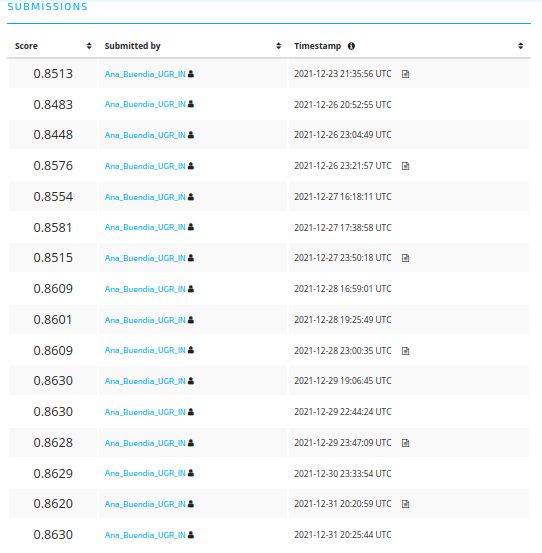
\includegraphics[scale=1]{submissions.png}
\caption{Tabla de submissions de DrivenData}
\end{figure}

\newpage
\tableofcontents
\newpage

\chapter{Práctica 3}
\section{Introducción}

Para la realización de esta práctica se ha participado en la competición de DrivenData \href{https://www.drivendata.org/competitions/66/flu-shot-learning/}{Flu Shot Learning: Predict H1N1 and Seasonal Flu Vaccines}.

El objetivo de la competición es predecir si una persona se ha vacunado con la vacuna de H1N1 o la vacuna de la gripe estacional usando 36 atributos distintos, siendo estos tanto categóricos como ordinales. Cabe destacar que algunos atributos, como respondent\_id, solo sirven para identificar el ejemplo.

El conjunto de entrenamiento consta de $26707$ instancias con sus etiquetas:

\begin{itemize}
\item \textbf{h1n1\_vaccine}: Indica si la persona está vacunada contra el H1N1 (1) o no (0).
\item \textbf{seasonal\_vaccine}: Indica si la persona está vacunada contra la gripe estacional (1) o no (0).
\end{itemize}

Como método de evaluación se usará el área bajo la curva ROC (AUC) para cada una de las variables, siendo la media de estas la puntuación obtenida.

\newpage
\section{Estructura}
El primer archivo de subida es \textit{ejemplo\_flu.py}, proporcionado por los profesores, con su correspondiente submission \textit{submission\_ejemplo\_flu\_rf.csv}. Cada uno de ellos se encuentra en su carpeta correspondiente: los archivos fuente se encuentran en \textit{src} (contiene archivos numerados de submissions) y sus correspondientes resultados se encuentran análogamente numerados en la carpeta \textit{submission}.

Además, en el directorio raíz se encuentra este documento de memoria de la práctica, así como el archivo excel editable y su exportación a pdf de la tabla resumen de subidas y la captura de pantalla de las submissions en DrivenData.
´
\newpage
\section{Exploración de los datos}

El primer paso en la commpetición es analizar el conjunto de datos y como está distribuido para entender mejor el problema y poder abordarlo de forma eficaz.

\subsection{Balanceo de clases}

Comenzamos comparando si las clases de nuestro problema están balanceadas o no, ya que si no lo están puede influir mucho en los clasificadores.

\begin{figure}[H]
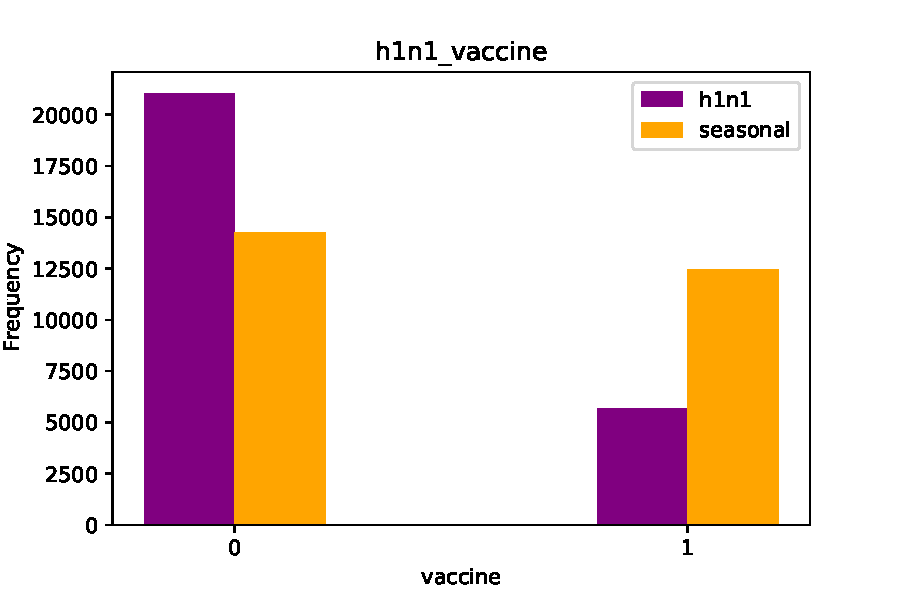
\includegraphics[scale=1]{desbalanceo.pdf}
\caption{Desbalanceo entre las vacunas}
\label{desbalanceo}
\end{figure}

Observamos en \eqref{desbalanceo} que la clase de las vacunas estacionales está más o menos balanceada, mientras que muy poca gente se ha vacunado de h1n1.

\subsection{Correlaciones}

Vamos a representar también un heatmap que muestre las correlaciones entre las distintas variables y las vacunas, para así tener una idea aproximada de qué variables proporcionan información similar y cuáles pueden ser mejores predictores de las vacunas.

\begin{figure}[H]
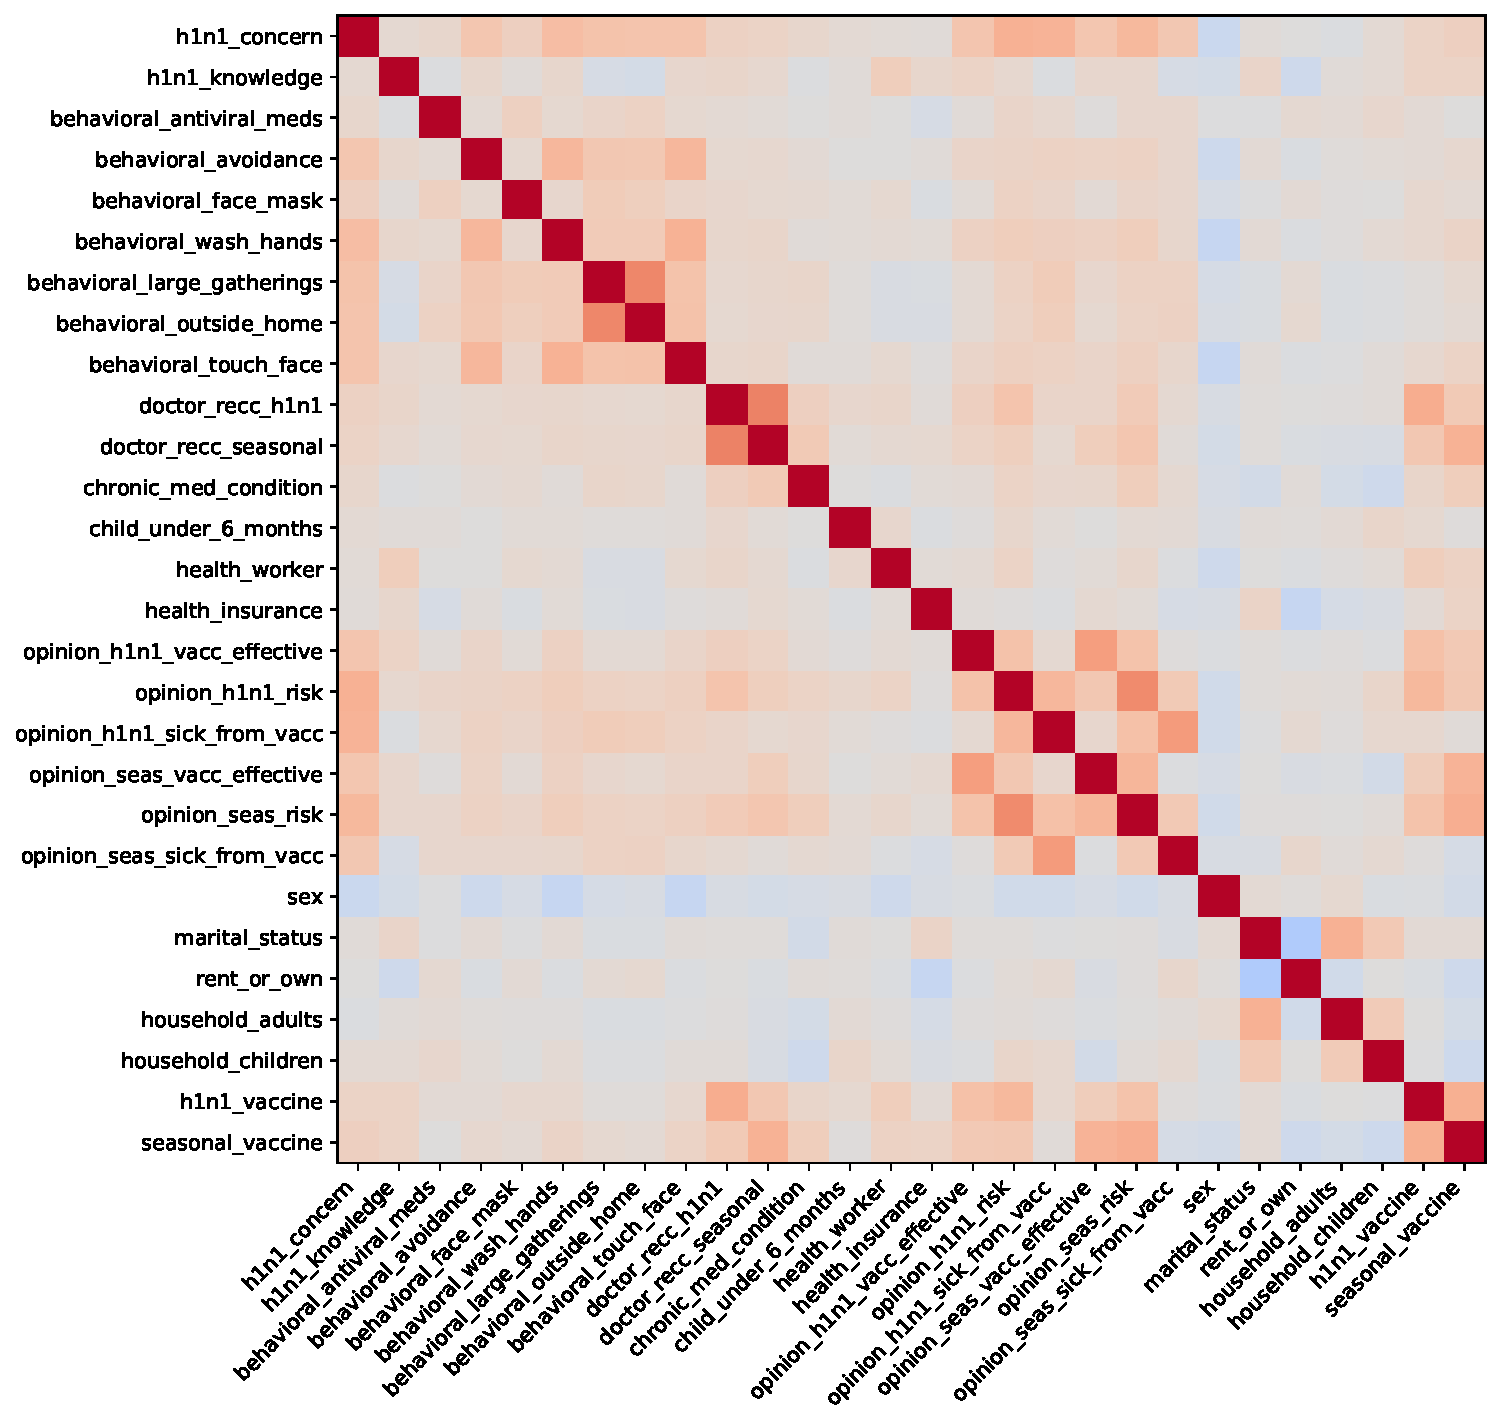
\includegraphics[scale=0.5]{correlaciones.pdf}
\caption{Correlaciones entre las variables y las clases}
\label{correlaciones}
\end{figure}

En \eqref{correlaciones} lo primero que llama la atención es como ambas vacunas están correlacionadas.

Además, vemos varias agrupaciones con correlación bastante alta, como por ejemplo todo el cúmulo de variables de las opiniones, las recomendaciones de los médicos sobre si ponerse o no una vacuna o todas las variables de comportamientos (lavarse las manos, evitar aglomeraciones etc).

Nos fijamos en que las recomendaciones de los doctores de vacunarse están muy relacionadas con ponerse las vacunas, al igual que las opiniones de los riesgos.

\subsection{Características}

Mirando el conjunto de características es claro que hay muchos valores perdidos, y, de cara al preprocesado, es necesario comprender la distribución de estas variables para realizar una buena imputacion de valores.

Comenzamos analizando qué códigos de empleo e industria se corresponden con trabajadores de la salud, con el fin de hacer una imputación más correcta.

\begin{figure}[H]
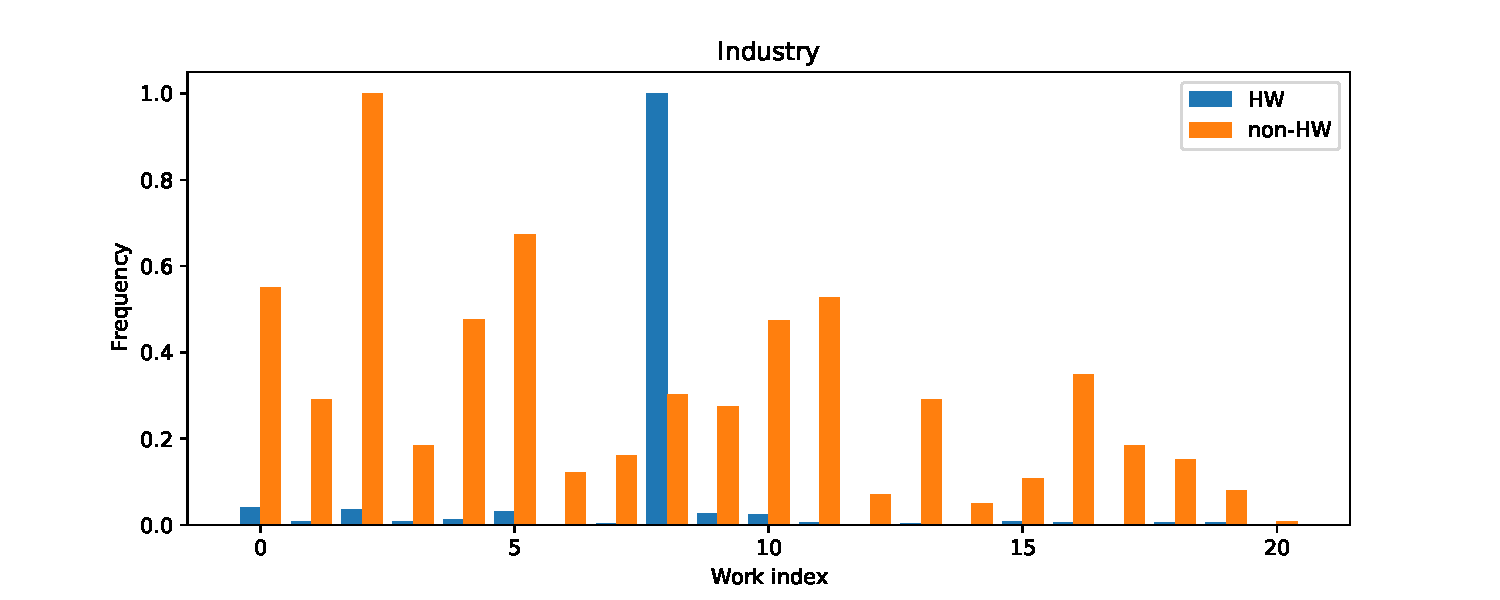
\includegraphics[scale=0.5]{industry.pdf}
\caption{Industrias en las que trabajan sanitarios y no sanitarios}
\label{industry}
\end{figure}

\begin{figure}[H]
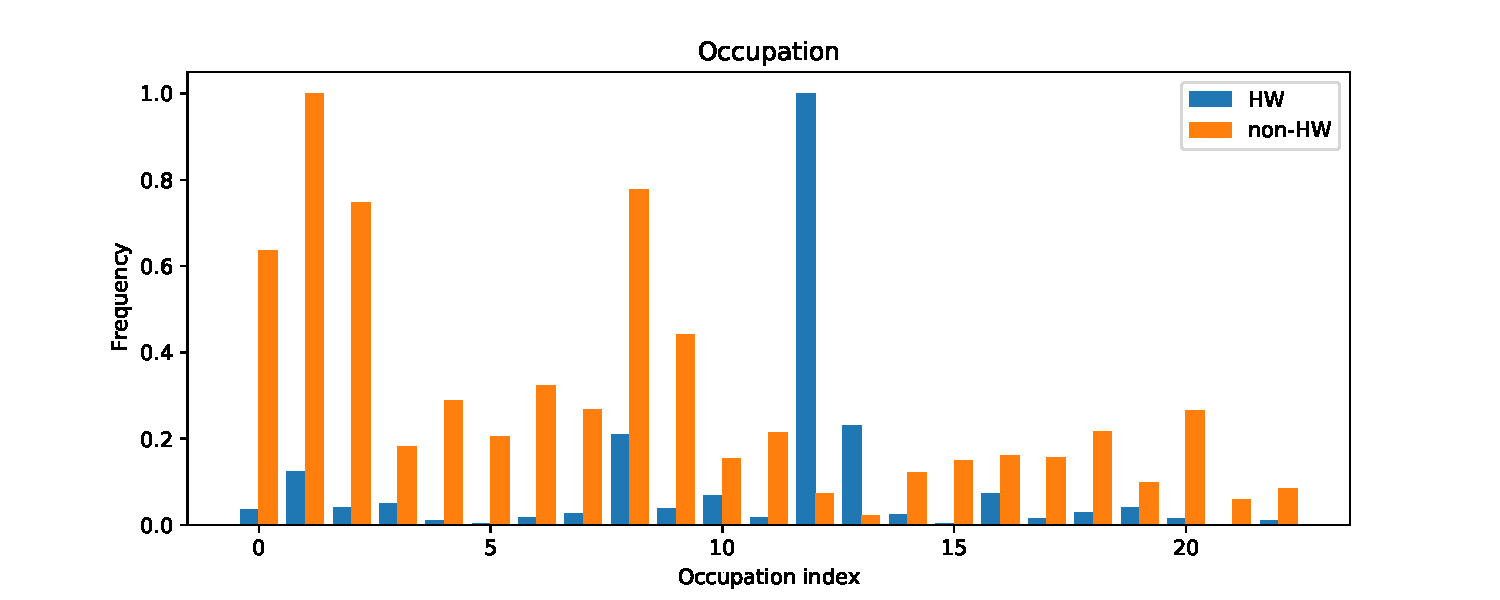
\includegraphics[scale=0.5]{occupation.pdf}
\caption{Ocupación de sanitarios y no sanitarios}
\label{occupation}
\end{figure}

Como vemos en \eqref{industry} y \eqref{occupation}, los sanitarios están en muchas industrias, pero sobre todo están en una de ellas, al igual que sucede con la ocupación. Por tanto, cada vez que tengamos un sanitario con empleo desconocido, parece razonable asignar esas etiquetas.

Además, muchos de los valores perdidos en industria y ocupación se encuentran en personas en desempleo o que no están en busca de empleo. Vamos a analizar también la correlación entre no estar trabajando, así como su edad y ser sanitario:

\begin{figure}[H]
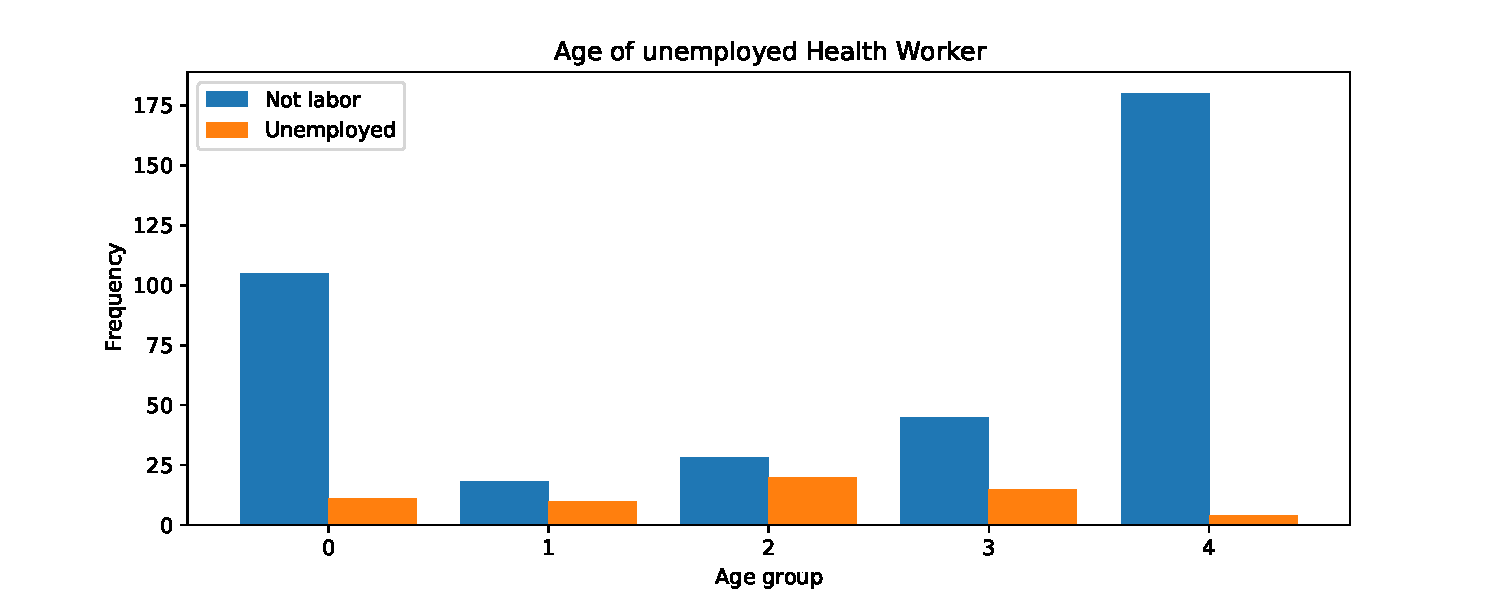
\includegraphics[scale=0.5]{edad_hw.pdf}
\caption{Estado de desempleados o sin buscar trabajo según edad de los sanitarios}
\label{edad_empleo_hw}
\end{figure}

Y comparamos los resultados con los de la población general:

\begin{figure}[H]
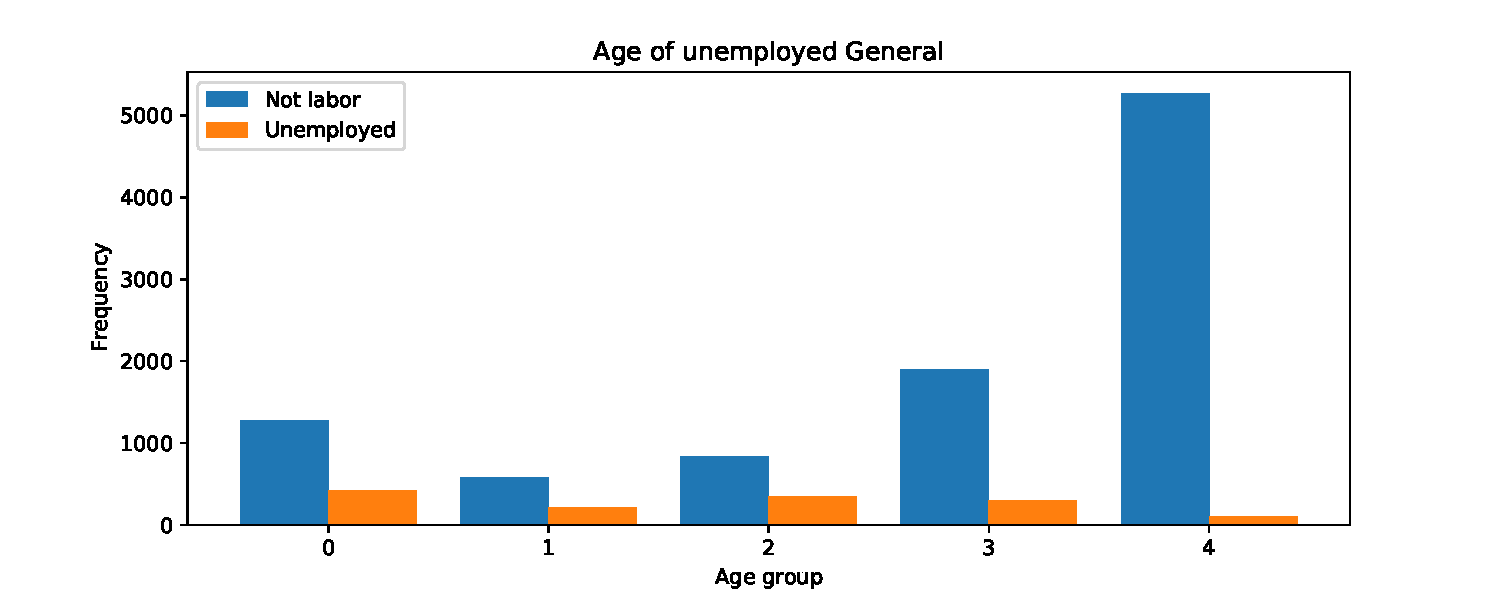
\includegraphics[scale=0.5]{unemployed_edad.pdf}
\caption{Estado de desempleados o sin buscar trabajo según edad de toda la población}
\label{edad_empleo}
\end{figure}

En \eqref{edad_empleo_hw} y \eqref{edad_empleo} se ve más o menos la misma tendencia, con quizá maás estudiantes en medicina que en general.

Estudiamos ahora el estado de empleo según la edad:

\begin{figure}[H]
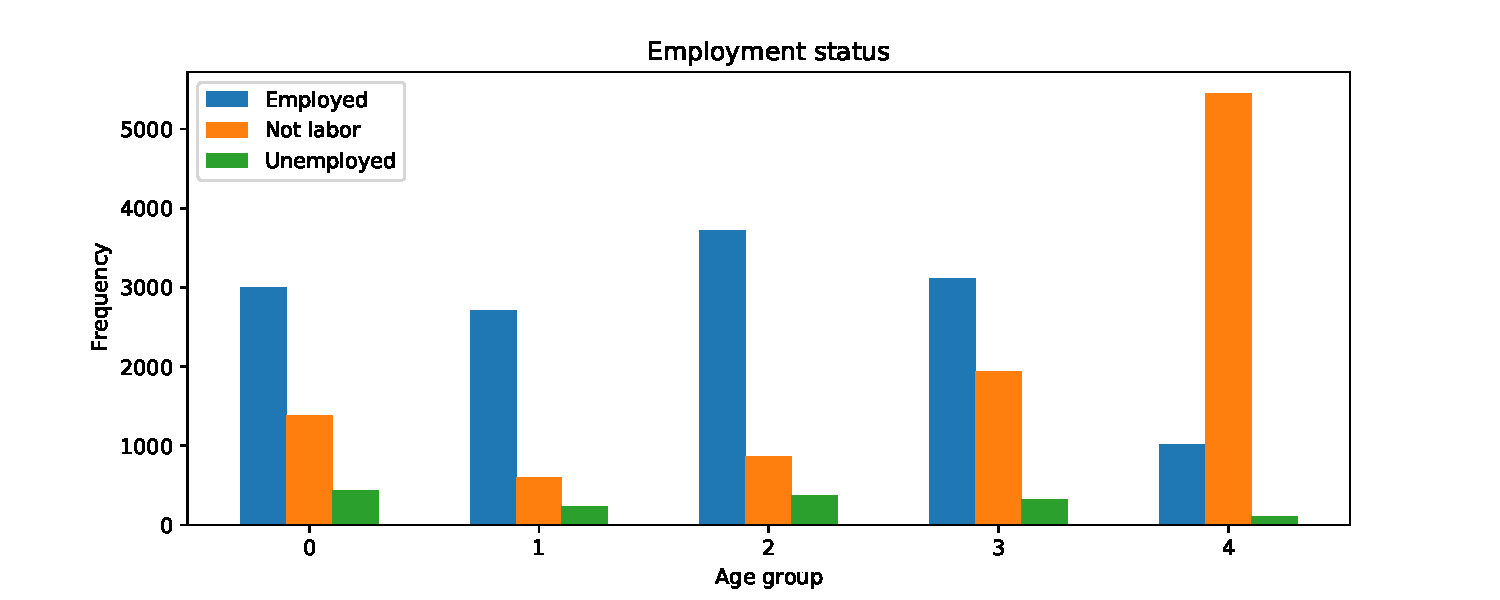
\includegraphics[scale=0.5]{employment_status_segun_age.pdf}
\caption{Estado de empleo según edad de toda la población}
\label{edad_empleo_completo}
\end{figure}

Observando \eqref{edad_empleo_completo} vemos que el desempleo es bajo para edades menores de 55 años y después sube. También hay muchos estudiantes en el primer grupo. ¿Estos grupos tienen ingresos? Realizamos otra representación para comprobarlo, ya que en las correlaciones parece una variable relevante.

\begin{figure}[H]
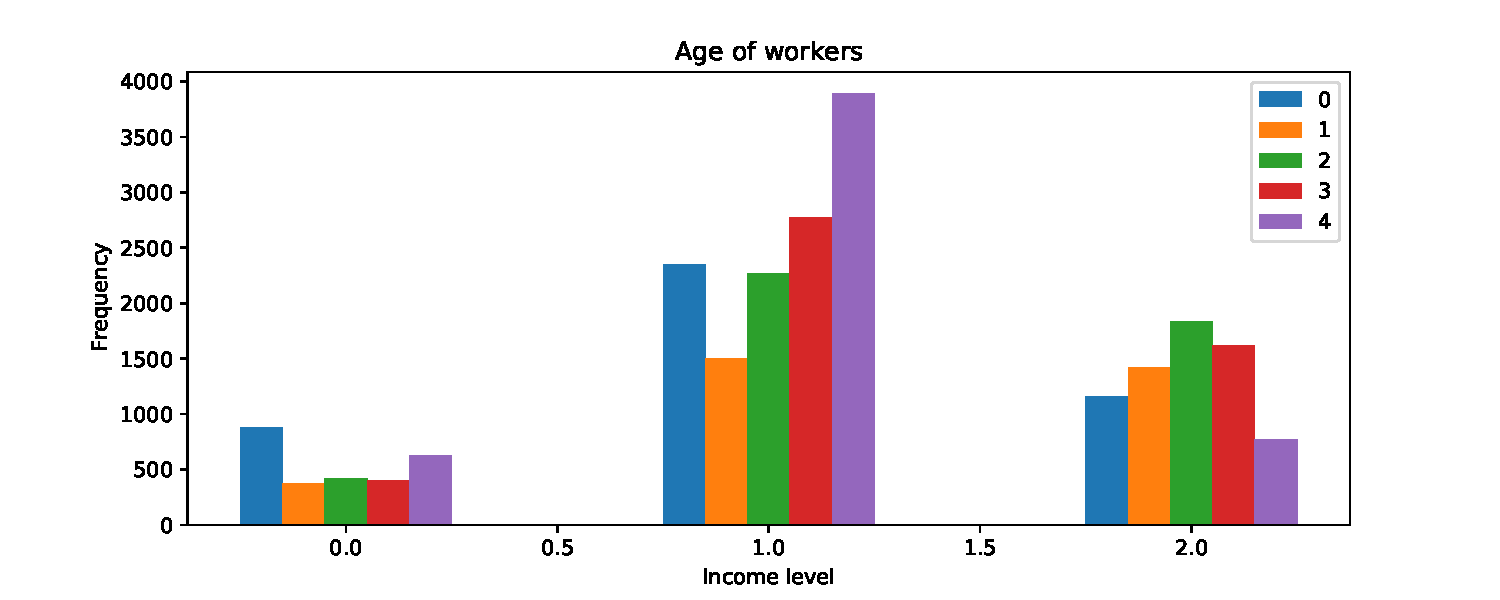
\includegraphics[scale=0.5]{edad_segun_income.pdf}
\caption{Ingresos según la edad}
\label{ingresos}
\end{figure}

En \eqref{ingresos} se confirma como las personas mayores tienen más ingresos quelas personas jóvenes, pero no parece aportar demasiada información relevante que podamos usar.

\newpage
\section{Progreso}

\subsection{Tabla de progresos}

\tiny
\begin{longtable}{|l|l|l|l|l|m{7em}|m{7em}|m{7em}|m{7em}|}

        Fecha & Hora(CET) & Posición & Sc. Train. & Sc. Test & Preprocesado & Algoritmos & Parámetros & Comentarios \\ \hline
        23/12/21 & 22:35:00 & 344 & 0.8543 & 0.8513 & Imputación de valores & Random forest & Por defecto & Fichero de prueba del profesor \\ \hline
        26/12/21 & 20:52:00 & 344 & 0.8589 & 0.8483 & Eliminando instancias con muchos nulos  e imputación de valores simple & Random forest & Por defecto & ~ \\ \hline
        27/12/21 & 00:04:00 & 344 & 0.8502 & 0.8448 & Imputación de valores simple & CatboostClassifier & Iterations 10, depth 2, learning\_rate 1 & Probando el catboost \\ \hline
        27/12/21 & 00:21:00 & 322 & 0.8624 & 0.8576 & Imputación de valores simple & CatboostClassifier & Iterations 45, depth 6 & Ajustados parámetros de catboost para resultado óptimo \\ \hline
        27/12/21 & 17:15:00 & 322 & 0.8609 & 0.8554 & Imputación de valores simple & Random forest & n\_estimators 300, min\_samples\_split 35, min\_samples\_leaf 3  & Pruebo ajuste parámetros de RF \\ \hline
        27/12/21 & 18:39:00 & 320 & 0.8656 & 0.8581 & Imputación de valores simple & CatboostClassifier & Iterations 45, depth 6 learning\_rate 0.31 & Añado otro paremtro a catboost \\ \hline
        28/12/21 & 00:50:00 & 320 & 0.8583 & 0.8515 & Imputación de valores simple & CatboostClassifier & Iterations 70, depth6,  learning rate 0.31 weights todo a 1 salvo las reccomendations a 2 & No quería subir esa :’) \\ \hline
        28/12/21 & 17:59:00 & 213 & 0.8669 & 0.8609 & Imputación de valores simple & LGBM & n\_estimators=100, learning\_rate=0.072, num\_leaves=29, min\_child\_samples=110 & Probando LGBM con parametros \\ \hline
        28/12/21 & 20:25:00 & 213 & 0.8708 & 0.8601 & Imputaciónd de valores simple y oversampling de 2000 instancias & LGBM & n\_estimators=100, learning\_rate=0.072, num\_leaves=29, min\_child\_samples=111 & Pruebo a hacer oversampling, ha ido mejor de lo esperado \\ \hline
        29/12/21 & 00:00:00 & 214 & 0.8675 & 0.8609 & Imputación de valores simple y undersampling de 200 instancias & LGBM & n\_estimators=100, learning\_rate=0.072, num\_leaves=29, min\_child\_samples=112 & Pruebo el undersampling (la hora esta bien, ha sido a las 00 justas) \\ \hline
        29/12/21 & 20:06:00 & 68 & 0.8683 & 0.8630 & Imputacion de valores simple & LGBM & boosting\_type="goss", top\_rate=0.42, max\_depth=0, subsample\_for\_bin=3000, n\_estimators=2500, learning\_rate=0.005, num\_leaves=29, min\_child\_samples=100 & Ajusto parametros \\ \hline
        29/12/21 & 23:44:00 & 69 & 0.8683 & 0.8630 & Imputacion de valores simple & LGBM & boosting\_type="goss", top\_rate=0.42, max\_depth=0, subsample\_for\_bin=3000, n\_estimators=2500, learning\_rate=0.005, num\_leaves=29, min\_child\_samples=100, path\_smooth=10 & Intento mejorar parametros \\ \hline
        30/12/21 & 00:47:00 & 69 & 0.8682 & 0.8628 & Imputacion de valores inteligente & LGBM & boosting\_type="goss", top\_rate=0.42, max\_depth=0, subsample\_for\_bin=3000, n\_estimators=2500, learning\_rate=0.005, num\_leaves=29, min\_child\_samples=100, path\_smooth=10 & Intento otro preprocesado sin éxito \\ \hline
        31/12/21 & 00:33:00 & 69 & 0.8684 & 0.8629 & Imputación de valores inteligente mejorada & LGBM & boosting\_type="goss", top\_rate=0.42, max\_depth=0, subsample\_for\_bin=3000, n\_estimators=2500, learning\_rate=0.005, num\_leaves=29, min\_child\_samples=100, path\_smooth=10 & Intento otro preprocesado sin éxito \\ \hline
        31/12/21 & 21:20:00 & 69 & 0.8675 & 0.8620 & Imputacion de valores simple y normalizacion & LGBM & boosting\_type="goss", top\_rate=0.42, max\_depth=0, subsample\_for\_bin=3000, n\_estimators=2500, learning\_rate=0.005, num\_leaves=29, min\_child\_samples=100, path\_smooth=11 & Intento preprocesado sin xito \\ \hline
        31/12/21 & 21:25:00 & 69 & 0.8683 & 0.8630 & Imputacion de valores simple y normalizacion & LGBM & boosting\_type="goss", top\_rate=0.42, max\_depth=0, subsample\_for\_bin=3000, n\_estimators=2500, learning\_rate=0.005, num\_leaves=29, min\_child\_samples=100, path\_smooth=12 & Intento normalizar de nuev o sin éxito \\ \hline

\caption{Submissions realizadas. Puede consultarse en el excel adjunto. Mejor marca $0.8630$ en posición $69$}
\label{tabla}

\end{longtable}

\normalsize

\subsection{Avances}

La primera entrega fue el fichero proporcionado por los profesores que usa random forest, se usó sin ninguna modificación para probar el sistema de subidas y marcar la medida a superar con las siguientes subidas. En este fichero el único preprocesado consiste en imputar todos los valores perdidos por el más frecuente, y es a lo que nos referiremos de ahora en adelante como imputación de valores simple.

A partir de este fichero, todas las entregas están nombradas como submission<numero>.py y su correspondiente .csv para su fácil identificación.

En segundo lugar se probó un preprocesado en el que se eliminaban todas las instancias con más de tres valores nulos en la misma fila, para comprobar si mejoraba el rendimiento del algoritmo, pero no fue así. Igualmente tampoco mejoró al eliminar algunas columnas que tenían gran cantidad de valores perdidos, como industry u occupation.

Después, dado que en la primera práctica el algoritmo XGBoost dio buen resultado, se ha probado la implementación de CatBoostClassifier, ya que trabaja bien con variables categóricas. Esta subida fue solamente el algoritmo, y en la siguiente se cambiaron los parámetros del mismo para mejorar la marca.

Dado que el resultado mejoró notablemente al cambiar los parámetros, se volvió al algoritmo random forest y se probó a modificar los parámetros allí para la siguiente subida.

Como no se mejoraron los resultados obtenidos por CatBoostClassifier, se volvió a este clasificador y se probaron más combinaciones de parámetros en las dos siguientes subidas, sin lograr mejorar la marca.

Con este algoritmo, aunque no se realizaron subidas ya que bajaba el score incluso en training, se han probado los métodos de smote, oversampling y undersampling, así como normalización minmax y standard usando las herramientas de sklearn.

Como ninguno de los preprocesados probados ha funcionado, probé el LGBMClassifier habiendo modificado los parámetros.

También, pese a que bajaba ligeramente el training probé a subir a drivendata los resultados de aplicar oversampling y undersampling por si reducían overfitting, pero no fue así.

Se probó entonces a cambiar el método de imputación de valores a la media en las variables ordinales, pero no mejoró, así como se probaron también de sklearn el KNNImputer y el IterativeImputer con distintos métodos predictivos y parámetros cada uno, pero de nuevo bajaron el score en training. Asimismo se volvió a incluir la normalización minmax y standard, pero tampoco mejoraban el resultado. Así, ninguna submission de drivendata cuenta con estos métodos, a pesar de que se ha trabajado en ellos.

\begin{figure}[H]
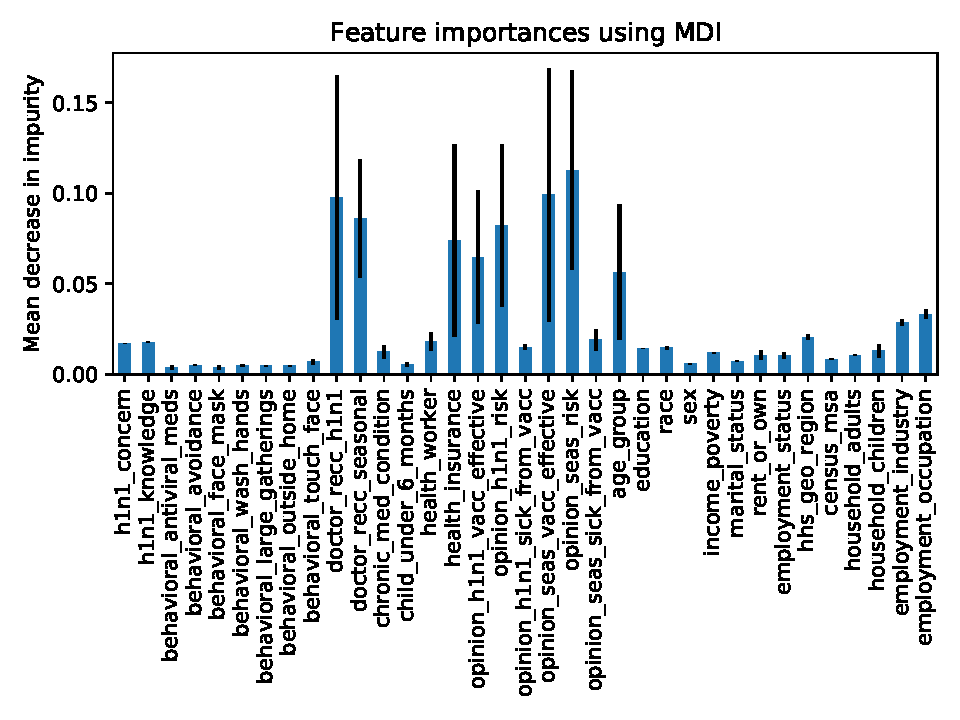
\includegraphics[scale=1]{atributos.pdf}
\caption{Importancia de los atributos según random forest}
\label{arbol}
\end{figure}

Asimismo, se probó a modificar la importancia de las variables basándonos en la relevancia de cada una de ellas, obtenidas a partir del clasificador RandomForest, como se muestra en \eqref{arbol}.

Por tanto, las dos siguientes entregas de nuevo fueron modificar los parámetros de LGBMClassifier, obteniendo así 0.8630, que es la puntuación más alta que se ha alcanzado.

Finalmente se volvió a intentar con distintos preprocesados, donde destaca la imputación de valores a la que en la tabla nos referimos como "\textbf{imputación de valores inteligente}", pues se basa en la exploración de datos realizada antes.

En este preprocesado las personas que sean sanitarios aparecerán como empleados (employment\_status) y los códigos de industry y occupation son los que se dan con más frecuencia en los sanitarios, vistos antes.

Además, si alguien está desempleado, como valor en su industry y occupation aparecerá "no trabaja" si los campos no están rellenos, variable global de sustitución.

De igual manera, si su estado es "not in labor force" se rellena con "no procede".

Los valores perdidos restantes se rellenan con el valor  más frecuente distinto de estás variables globales.

El código es el siguiente:

\begin{verbatim}
no_empleado = "no empleado"
no_procede = "no procede"
empleado_healthcare_industry = "fcxhlnwr"
empleado_healthcare_occupation = "cmhcxjea"

mask_no_empleado_health = (data_x['health_worker'] == 1) & 
(data_x['employment_status'] == "Unemployed") & (data_x['employment_industry'].isna())
data_x_tmp = data_x

mask = (data_x["health_worker"] == 1) &  data_x["employment_status"].isna() 
data_x_tmp.loc[mask, "employment_status"] = "Employed" 

mask = (data_x_tst["health_worker"] == 1) &  data_x_tst["employment_status"].isna() 
data_x_tst.loc[mask, "employment_status"] = "Employed" 

mask =  ~data_x_tmp["employment_status"].isna() 

data_y = data_y.mask(mask)
data_x_tmp = data_x_tmp.mask(mask)
data_x_tmp.loc[mask, "employment_status"] = "unknown"

mask = data_x_tst["employment_status"].isna() 
data_x_tst.drop(data_x_tst[mask].index, inplace=True)
data_x_tst.loc[mask, "employment_status"] = "unknown"

for hwdata, col in zip([empleado_healthcare_industry, empleado_healthcare_occupation],
["employment_industry", "employment_occupation"]):

    mask = (data_x["health_worker"] == 1) & 
    (data_x["employment_status"] == "Employed") & (data_x[col].isna())
    data_x_tmp.loc[mask, col] = hwdata

    mask = (data_x_tst["health_worker"] == 1) & 
    (data_x_tst["employment_status"] == "Employed") & (data_x_tst[col].isna())
    data_x_tst.loc[mask, col] = hwdata

    mask = (data_x['employment_status'] == "Unemployed") & 
    (data_x[col].isna())
    data_x_tmp.loc[mask, col] = no_empleado

    mask = (data_x_tst['employment_status'] == "Unemployed") & 
    (data_x_tst[col].isna())
    data_x_tst.loc[mask, col] = no_empleado

    mask = (data_x['employment_status'] == "Not in Labor Force") & 
    (data_x[col].isna())
    data_x_tmp.loc[mask, col] = no_procede

    mask = (data_x_tst['employment_status'] == "Not in Labor Force") & 
    (data_x_tst[col].isna())
    data_x_tst.loc[mask, col] = no_procede

    mask = data_x_tmp[col].isna()
    data_x_tmp.loc[mask, col] = "unknown"
    mask = data_x_tst[col].isna()
    data_x_tst.loc[mask, col] = "unknown"'''
    
    most_frequent = data_x_tmp[col].value_counts().index
    selected = 0

    while most_frequent[selected] == no_procede or
     most_frequent[selected] == no_empleado or most_frequent[selected] == hwdata:
        selected += 1
        
    data_x_tmp[col].fillna(most_frequent[selected], inplace=True)
    data_x_tst[col].fillna(most_frequent[selected], inplace=True)
\end{verbatim}

\newpage
\section{Herramientas con las que se ha trabajado}

\begin{itemize}
\item RandomForest classifier
\item CatBoostClassifier
\item LGBMClassifier
\item sklearn.preprocessing SimpleImputer
\item sklearn.preprocessing KNNImputer
\item sklearn.preprocessing IterativeImputer
\item sklearn.preprocessing MinMaxScaler
\item sklearn.preprocessing StandardScaler
\item sklearn.preprocessing OneHotEncoder
\item sklearn.utils Resample
\item imblearn smote
\item sklearn.preprocessing LabelEncoder
\item sklearn.model\_selection Kfold
\item sklearn.multioutput MultiOutputClassifier


\end{itemize}




% ----------------------- %
% BIBLIOGRAFÍA
% ----------------------- %

% Estilo de cita.
%\usepackage{natbib} YA SE IMPORTA EN OTRO PUNTO, NO HACE FALTA PONERLO AQUI
% FUENTE CUSTOM
%\bibliographystyle{apa-good}
% formato de citas original
\newpage
\bibliographystyle{unsrtnat}

\chapter{Bibliografía}
\begin{itemize}
\item Diapositivas de la asignatura.
\item \href{https://pandas.pydata.org/docs/}{https://pandas.pydata.org/docs/}
\item \href{https://matplotlib.org/}{https://matplotlib.org/}
\item \href{https://scikit-learn.org/stable/}{https://scikit-learn.org/stable/}
\item \href{https://catboost.ai/en/docs/concepts/python-reference\_catboostclassifier}{https://catboost.ai/en/docs/concepts/python-reference\_catboostclassifier}
\item \href{https://lightgbm.readthedocs.io/en/latest/pythonapi/lightgbm.LGBMClassifier.html}{https://lightgbm.readthedocs.io/en/latest/pythonapi/lightgbm.LGBMClassifier.html}
\end{itemize}

\bibliography{bib/library}

\end{document}